\documentclass{mipt-thesis-bs}
% Следующие две строки нужны только для biblatex. Для inline-библиографии их следует убрать.
\usepackage{mipt-thesis-biblatex}
\usepackage{amsmath}
\usepackage[nottoc,notlot,notlof]{tocbibind}
\usepackage{tocloft}
\usepackage[backend=biber]{biblatex} 
\usepackage{graphicx}
\usepackage{hyperref}
		
%Some customization of hyperref	
		
\addbibresource{main.bib}

\title{Применение методов машинного обучения в задаче радиометрической классификации}
\author{Кайдаш А.\,А.}
\supervisor{Дворкович А.\,В.}
%\referee{Петров Д.\,Е.}       % требуется только для mipt-thesis-ms
\groupnum{Б01-813б}
\faculty{Физтех-школа Радиотехники и Компьютерных Технологий}
\department{Кафедра мультимедийных технологий и телекоммуникаций}

\begin{document}

\frontmatter
\titlecontents
\mainmatter

%\input{chapters/abbreviations}

\chapter{Введение}
\label{chap:intro}
	\paragraph{Актуальность проблемы} 
	\noindent \\
    	При столь быстром развитии технологий передачи сигналов появляется необходимость также и в развитии технологий детектирования устройств. Существуют методы, используемые для распознавания устройств на высших уровнях, но потребность в достаточном уровне защиты и точности все еще актуальна. 
	
	\paragraph{Цель работы}
	\noindent\\
	    Для обеспечения защиты информации необходимо с высокой точностью распознавать устройства.
	    
	\paragraph{Задачи} 
	\noindent 
	\begin{itemize}
	    \item Выбор эффективного признакового описания
	    \item Выбор алгоритмов классификации в режиме обучения с учителем
	    \item Разработка и реализация алгоритма онлайн-классификации
	\end{itemize}
    	То есть, разработка алгоритма, который по сигналу с передатчика сможет идентифицировать передающее устройство.
    	
	\paragraph{Объект исследования}
	\noindent \\
    	Задача радиометрической идентификации – выделение уникального набора шумов для использования их в качестве идентификатора устройства.
    	
	\paragraph{Предмет исследования} 
	\noindent \\
    	RF fingerprint – особая форма высокочастотного сигнала, которая зависит от конкретного передающего устройства. Данный сигнал представляет из себя шум, обусловленный внутренним устройством передатчика. На практике это сигнал, полученный путем анализа преамбул принятого сигнала.
    \newpage	
	\paragraph{Практическая значимость} 
	\noindent \\
    	Радиометрическая идентификация, в отличие от других методов защиты, использует для распознавания именно самый низкий, физический уровень, поэтому обеспечивает большую безопасность, чем алгоритмы распознавания, которые осуществляются на более высоких уровнях стека сетевых протоколов OSI.
        RF fingerprint – уникальный для каждого устройства набор шумов, его практически невозможно подделать, а значит он может быть использован для предотвращения различных сетевых атак, например, MITM.

	
	

\chapter{Обзор предметной области}
\label{chap:obzor}

    \section{Обозначения и сокращения} 
        \noindent\\
	    \textbf{RF} -- Radio Frequency \\
	    \textbf{RF-fingerprint} -- Radio Frequency Fingerprint \\
	    \textbf{MITM} -- Man In The Middle \\
	    \textbf{OFDM} -- Orthogonal Frequency-Division Multiplexing \\
	    \textbf{AE} -- Autoencoder\\
	    \textbf{RAW} -- Cырой, необработанный [сигнал]\\
        \textbf{ML} -- Machine Learning\\
	    \textbf{DT} -- Decision Tree\\
	    \textbf{TSNE (t-SNE)} -- t-distributed Stochastic Neighbor Embedding\\
	    \textbf{OSI} -- The Open Systems Interconnection model\\
	    \textbf{AGS} -- Automatic Gain Control\\
	    \textbf{DL} -- Deep Learning\\

    \newpage
    \section{Формальная запись проблемы}
        \par
            Сформулировать проблему можно так – необходимо с высокой точностью распознавать на физическом уровне устройства, сигнал которых мы уже принимали. \\
        \par
            Идентификация должна происходить вне зависимости от их конкретного расположения в пространстве, условий среды и зашумленности сигнала, а также с минимумом известных данных о конкретном устройстве. \\
        
        \par
            Ввиду своих физических свойств, – в случае OFDM, из-за преобразователей, усилителей и фильтров в схеме, – каждое передающее устройство уникально искажает сигнал. \\
            
            \begin{figure}[h!]
                \centering
                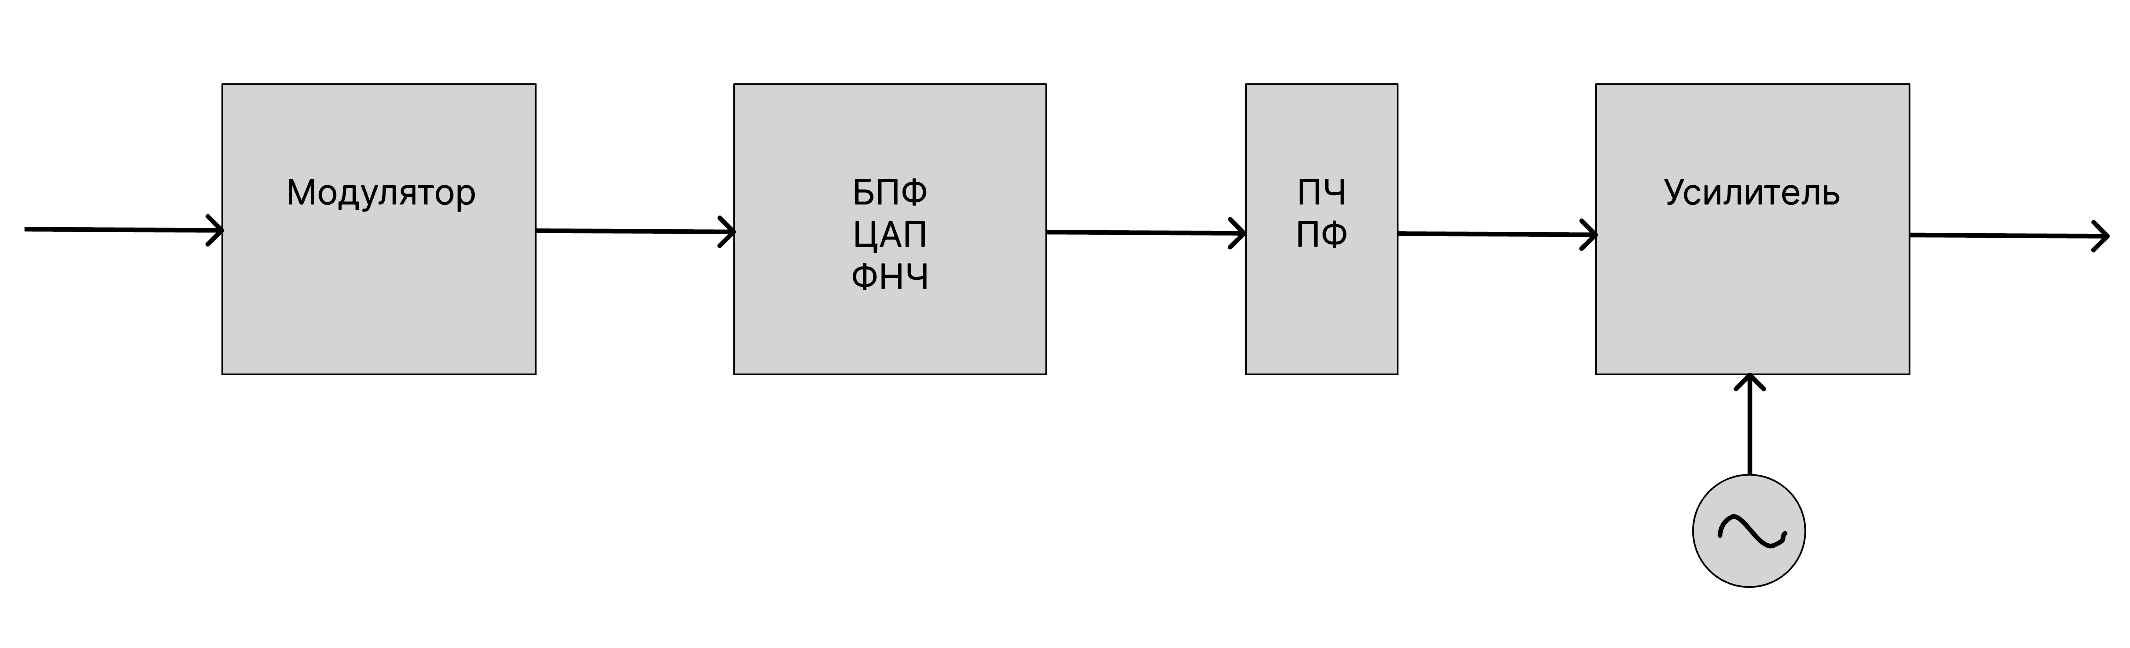
\includegraphics[scale=0.45]{pictures/index.png}
                \caption{Схема формирования OFDM-сигнала}
                \label{fig:my_label}
            \end{figure} 
            
        \par
            Для того, чтобы обнаружить внесенные искажения, необходимо выделить постоянные составляющие сигнала – преамбулы, после чего обработать их и решить задачу классификации на полученных данных.\\
            
            \begin{figure}[h!]
                \centering
                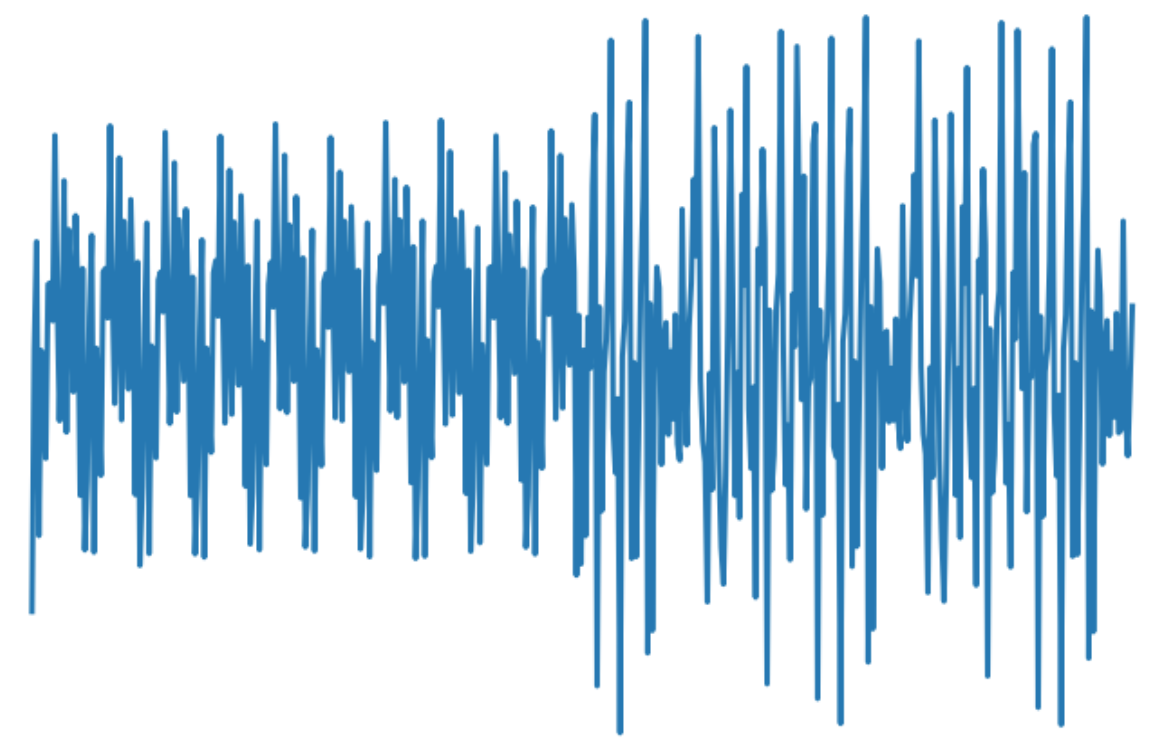
\includegraphics[scale=0.5]{pictures/preambules.png}
                \caption{Legacy преамбула}
                \label{fig:my_label}
            \end{figure} 
        \newpage
        \par
            В сигнале на Рис. 2 можно увидеть два поля legacy преамбулы: первая состоит из 10 одинаковых частей, а вторая из 2,5 одинаковых частей, с циклически расположенной начальной частью.
            \begin{figure}[h!]
                \centering
                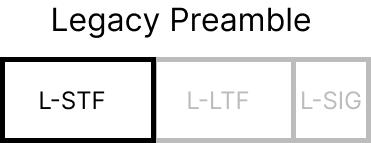
\includegraphics[scale=0.5]{pictures/L-STF.png}
                \caption{L-STF}
                \label{fig:my_label}
            \end{figure} 
        \par
            L-STF -- the Legacy short training field -- это первое поле 802.11 OFDM PLCP legacy преамбулы. \\
            \noindent
            Длительность L-STF зависит от полосы частот канала и составляет 8, 16 и 32 $\mu s$ для частот 20, 10 и 5 MHz соответственно.\\
            \noindent
            L-STF обладает хорошими корелляционными свойствами, поэтому используется для детекции начала пакетов, грубой частотной коррекции и установки AGC.\\
        \par
            \begin{figure}[h!]
                \centering
                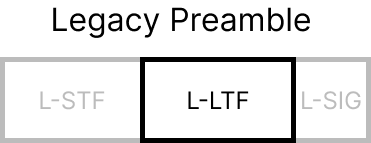
\includegraphics[scale=0.5]{pictures/L-LTF.png}
                \caption{L-LTF}
                \label{fig:my_label}
            \end{figure} 
            L-LTF -- the legacy long training field -- второе поле 802.11 OFDM PLCP legacy преамбулы.\\
            \noindent
            Длительность L-LTF также зависит от полосы частот канала и составляет 8, 16 и 32 $\mu s$ для частот 20, 10 и 5 MHz соответственно.\\
            \noindent
            L-LTF используется для оценки канала, точной оценки частотного смещения и точной оценки смещения символьной скорости.\\
        \newpage
            \begin{figure}[h!]
                \centering
                
\includegraphics[scale=0.4]{pictures/L-LTF-1.png}
                \caption{Устройство L-LTF}
                \label{fig:my_label}
            \end{figure} 
        
        \par
            L-LTF состоит из циклического префикса (CP) и двух следующих друг за другом идентичных символов C1 и C2. CP имеет длительность в 2 раза меньшую, чем C1 и С2 и в точности повторяет вторую половину последнего во временной области. 
            
            
        
        \par
            При обработке сигнала для распознавания конкретного устройства в задаче радиометрической идентификации необходимо не только выделить особенности преамбул, но и избавиться от зашумленности сигнала, внесенной условиями среды. Именно поэтому при обработке RAW сигнала необходимо отобрать значимые для классификации признаки.
            
        \par
            
        
    \section{Постановка задачи}
    
        По RAW сигналам необходимо, пользуясь методами машинного обучения, решить задачу классификации -- распознавания каждого устройства, для которого ранее собиралась информация.
        
        
        
    
     




\chapter{Выбор метода решения}
\label{chap:methods}
    \section{Подходы к решению задачи}
    \par
        Для решения данной задачи предлагается действовать по данному алгоритму:
        \noindent
        \begin{enumerate}
            \item Предобработка данных
            \item Отбор признаков
            \item Решение задачи классификации
            \item Адаптация классификатора
        \end{enumerate}
        
        \begin{figure}[h!]
                \centering
                
\includegraphics[scale=0.7]{pictures/logic.png}
                \caption{Алгоритм решения}
                \label{fig:my_label}
            \end{figure} 
    \newpage
    \section{Формулировка требований к решению} \\
        \paragraph{Необходимые свойства решения:}
         \\
        \begin{itemize}
            \item Оптимальность по времени выполнения
            \item Реальные требования к вычислительной мощности обрабатывающего устройства
            \item Масштабируемость композиции алгоритмов
            \item Отсутствие вычислений для нового образца по всем данным
            \item Возможность объединения алгоритмов для потоковой обработки сигналов
            \item Возможность дообучения на неразмеченных данных
            \item Сохранение модели для дальнейшего использования
            \item Возможность классификации без хранения обработанных ранее данных \\ \\
        \end{itemize}
        
    \newpage    
    \section{Методы решения}
    
        \paragraph{Выбор алгоритма для преобразования RAW сигнала} 
            \noindent \\
            
            \noindent
            Есть несколько вариантов преобразований RAW сигнала, а также множество их комбинаций. \\ \\
            В данной работе рассмотрены:
            \begin{itemize}
                \item FFT -- Fast Fourier transform -- алгоритм ускоренного вычисления дискретного преобразования Фурье.\\
                Данный алгоритм, в отличие от прямого дискретного преобразования Фурье, выполняющегося за $O(N^2)$, имеет асимптотику $O(N log(N))$.
                \item Разложение сигнала на модуль и аргумент.
                \item Разложение на действительную и мнимую части. \\
            \end{itemize} \\
        \paragraph{Выбор алгоритма для уменьшения размерности}
        \noindent \\
    
            \noindent 
            Для данной задачи необходимо значительно уменьшить размерность признакового пространства, по минимуму потеряв важную информацию об RF-Fingerprint устройства.\\ \\ 
            Может понадобиться не просто убрать менее значимые признаки, а создавать композиции из имеющихся признаков для минимальных потерь. Этой способностью обладают автоэнкодеры на основе нейронных сетей. \\ \\
            В данной работе рассмотрены:
            \begin{itemize}
                \item Алгоритм проекции на 2-мерное признаковое пространство -- TSNE
                \item Отбор признаков с помощью алгоритма Random Forest
                \item Встроенный автоэнкодер MATLAB
                \item Автоэнкодер, построенный с помощью библиотеки tensorflow.keras
                \item Permutation importance из библиотеки sklearn.inspection \\
            \end{itemize}
            
    
        \paragraph{Выбор алгоритма для классификации}
        \noindent\\
        
            \noindent
            Для данной задачи необходимо достаточно точно классифицировать зашумленные данные, обладающие признаками со сложной внутренней зависимостью. \\ \\
            Алгоритмы классификации, которые подходят для решения данной задачи должны быть быстродействующими, нетривиальными и помехоустойчивыми. \\ \\
            В данной работе рассмотрены: 
            \begin{itemize}
                \item Decision Tree -- Решающее дерево -- алгоритм, основанный на разделении по значению признаков для построения дерева
                \item Random Forest -- Случайный лес -- композиция решающих деревьев, более устойчивая к переобучению
                \item Multilayer Perceptron -- полносвязная нейронная сеть построенная с помощью библиотеки sklearn.sknn
                \item CatBoostClassifier -- open source классификатор от компании Yandex
            \end{itemize}   
            
            %про всякие алгоритмы
\chapter{Описание метода решения}
\label{chap:def}
    \section{Математический аппарат} \\
    \paragraph{Метрики}
    \noindent \\
        
    \noindent
        В работе используются следующие метрики: \\
        \begin{enumerate}
            \item MultiClass:
             $$
            \sum_{i=1}^{N} w_{i} \log \left(\frac{e^{a_{i t_{i}}}}{\sum_{j=0}^{M-1} e^{a_{i j}}}\right)
            $$
            $$
            \sum_{i=1}^{N} w_{i}$$
            $$
            t \in\{0, \ldots, M-1\}
            $$
            \item MultiClassOneVsAll: 
            $$
            \frac{\frac{1}{M} \sum_{i=1}^{N} w_{i} \sum_{j=0}^{M-1}\left[j=t_{i}\right] \log \left(p_{i j}\right)+\left[j \neq t_{i}\right] \log \left(1-p_{i j}\right)}{\sum_{i=1}^{N} w_{i}}
            $$
            $$          
            t \in\{0, \ldots, M-1\}
            $$
            \item Total F1 weighted:
            $$ 
            \frac{\sum_{i=1}^{M} w_{i} F 1_{i}}{\sum_{i=1}^{M} w_{i}}
            $$
            \item MCC: 
            $$
            \frac{\sum_{k} \sum_{l} \sum_{m} C_{k k} C_{l m}-C_{k l} C_{m k}}{\sqrt{\sum_{k}\left(\sum_{l} C_{k l}\right)\left(\sum_{k^{\prime} \mid k^{\prime} \neq k} \sum_{l^{\prime}} C_{k^{\prime} l^{\prime}}\right)} \sqrt{\sum_{k}\left(\sum_{l} C_{l k}\right)\left(\sum_{k^{\prime} \mid k^{\prime} \neq k} \sum_{l^{\prime}} C_{l^{\prime} k^{\prime}}\right)}}
            $$
            \item Accuracy:
            $$
            \frac{\sum_{i=1}^{N} w_{i}\left[\operatorname{argmax}_{j=0, \ldots, M-1}\left(a_{i j}\right)==t_{i}\right]}{\sum_{i=1}^{N} w_{i}}
            $$
            $$
            t \in\{0, \ldots, M-1\}
            $$
            \item Hinge loss:
            $$
            \ell(y)=\max (0,1-t \cdot y)
            $$
            \item Hamming loss:
            $$
            \sum_{i=1}^{N} w_{i}\left[\operatorname{argmax}_{j=0, \ldots, M-1}\left(a_{i j}\right) \neq t_{i}\right]
            $$
            $$
            \sum_{i=1}^{N} w_{i}
            $$
            \item Zero One loss:
            $$1 - Accuracy$$
            \item Kappa:
            $$
            1-\frac{1-Accuracy }{1-RAccuracy }
            $$
$$RAccuracy =\frac{\sum_{k=0}^{M-1} n_{k_{a}} n_{k_{t}}}{\left(\sum_{i=1}^{N} w_{i}\right)^{2}}
$$
            \item WKappa:
            $$
\kappa_{w}=\frac{p_{o}-p_{e}}{1-p_{e}}
$$
где $p_{0}=\sum_{i=1}^{K} \sum_{j=1}^{K} w_{i j} p_{i j}$ и $p_{e}=\sum_{i=1}^{K} \sum_{j=1}^{K} w_{i j} p_{i . p} p_{. j}$ при $0 \leq w_{i j} \leq 1$ и $w_{j j}=1(i, j=1, \cdots, K)$, или
$$
\kappa_{w}=1-\frac{q_{o}}{q_{e}}
$$
где $q_{0}=\sum_{i=1}^{K} \sum_{j=1}^{K} v_{i j} p_{i j}$ и  $q_{e}=\sum_{i=1}^{K} \sum_{j=1}^{K} v_{i j} p_{i .} p_{. j}$ при $0 \leq v_{i j} \leq 1$ и $v_{j j}=0(i, j=1, \cdots, K)$. 
            \item AUC$\mu$:
            $$\mathrm{AUC}=\frac{1}{n_{+} n_{-}} \sum_{\hat{p}^{(i)} \in D^{+}} \sum_{\hat{p}^{(j)} \in D^{-}} \tilde{I}\left(\hat{p}^{(i)}-\hat{p}^{(j)}\right)$$
            $$S(i, j)=\frac{1}{n_{i} n_{j}} \sum_{a \in D^{i}, b \in D^{j}} \tilde{I} \circ O\left(\mathbf{y}^{(a)}, \mathbf{y}^{(b)}, \hat{\mathbf{p}}^{(a)}, \hat{\mathbf{p}}^{(b)}, \mathbf{v}_{i, j}\right)$$
            $$\mathrm{AUC}_{\mu}=\frac{2}{K(K-1)} \sum_{i<j} S(i, j)$$
        \end{enumerate}
        
        \newpage
        \paragraph
        {
        Метрический классификатор
        }
        \noindent\\
        
        \noindent
        Для произвольного объекта $a \in X$ расположим элементы обучающей выборки $x_{1}, \ldots, x_{\ell}$ в порядке возрастания расстояний до $a$ :
$$
\rho\left(a, x_{a}^{(1)}\right) \leqslant \rho\left(a, x_{a}^{(2)}\right) \leqslant \cdots \leqslant \rho\left(a, x_{a}^{(\ell)}\right)
$$
где через $x_{a}^{(i)}$ обозначается $i$-й сосед объекта $a$. Соответственно, ответ на $i$-м соседе объекта $a$ есть $y_{a}^{(i)}=y^{*}\left(x_{a}^{(i)}\right)$. Таким образом, любой объект $a \in X$ порождает свою перенумерацию выборки.

\emph{Определение.} Метрический алгоритм классификации с обучающей выборкой $X^{\ell}$ относит объект $x$ к тому классу $y \in Y$, для которого суммарный вес ближайших обучающих объектов $\Gamma_{y}\left(x, X^{\ell}\right)$ максимален:
$$
a\left(x ; X^{\ell}\right)=\arg \max _{y \in Y} \Gamma_{y}\left(x, X^{\ell}\right) ; \quad \Gamma_{y}\left(x, X^{\ell}\right)=\sum_{i=1}^{\ell}\left[y_{x}^{(i)}=y\right] w(i, x),
$$
где функция $w(i, x)$ оценивает степень важности $i$-го соседа для классификации объекта $x$. \\Функция $\Gamma_{y}\left(x, X^{\ell}\right)$ называется оценкой близости объекта $x$ к классу $y.$\cite{8}\\ 

        \paragraph
        {
        Линейный классификатор 
        }
        \noindent\\
        
        \noindent
        Пусть $X$ - пространство объектов; $Y=\{-1,1\}$ - множество допустимых ответов; объекты описываются $n$ числовыми признаками $f_{j}: X \rightarrow \mathbb{R}, j=1, \ldots, n$. Вектор $x=\left(x^{1}, \ldots, x^{n}\right) \in \mathbb{R}^{n}$, где $x^{j}=f_{j}(x)$, называется признаковым описанием объекта $x$.\\
        Если дискриминантная функция определяется как скалярное произведение вектора $x$ и вектора параметров $w \in \mathbb{R}^{n}$, то получается линейный классификатор:\cite{8}
$$
a(x, w)=\operatorname{sign}\left(\langle w, x\rangle-w_{0}\right)=\operatorname{sign}\left(\sum_{j=1}^{n} w_{j} f_{j}(x)-w_{0}\right)
$$ 
        \newpage
        \paragraph
        {
        Multilayer perceptron
        }
        \noindent\\
        
        
        Персептрон – линейный классификатор. Это математическая модель нейрона -- нервной клетки мозга. \\
        \begin{figure}[h!]
                \centering
                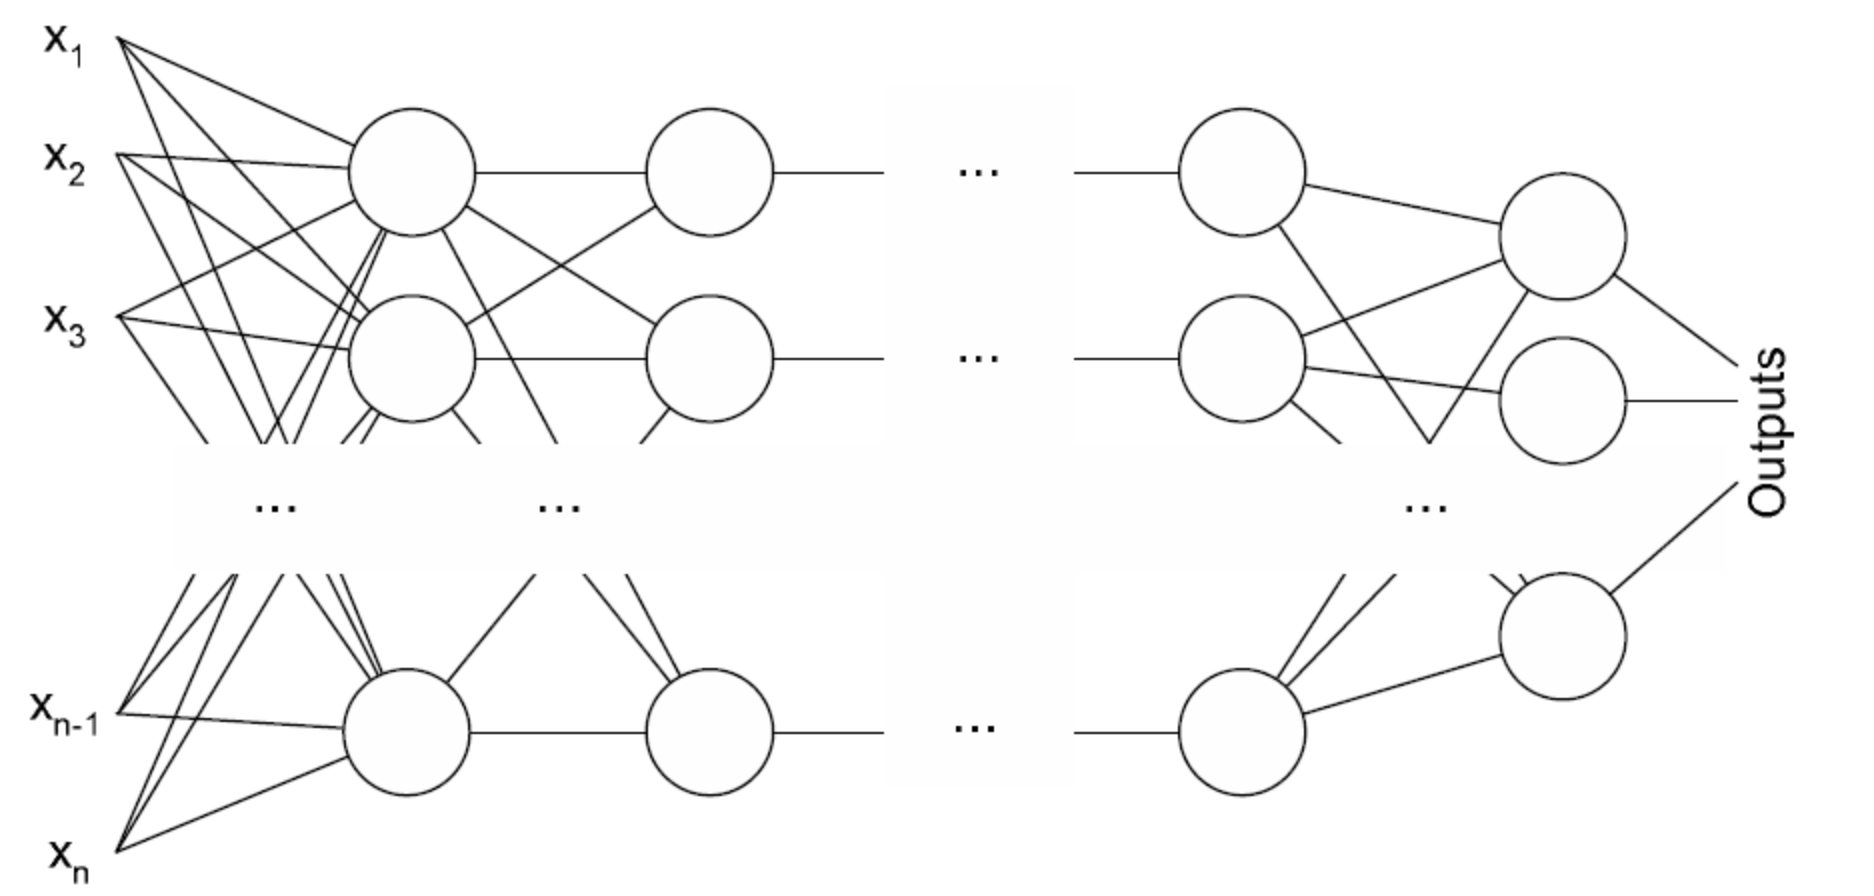
\includegraphics[scale=0.4]{pictures/perseptron.png}
                \caption{Multilayer perceptron}
                \label{fig:my_label}
            \end{figure} 
        \par
        Нейрон принимает каждый такт на свои n входов заряды величиной $x_j = f_j (x)$ . \\ 
        Эти заряды умножаются на веса $w_j$, а затем берется их сумма. У возбуждающего синапса положительный вес, а у тормозящего -- отрицательный. \\
        \begin{figure}[h!]
                \centering
                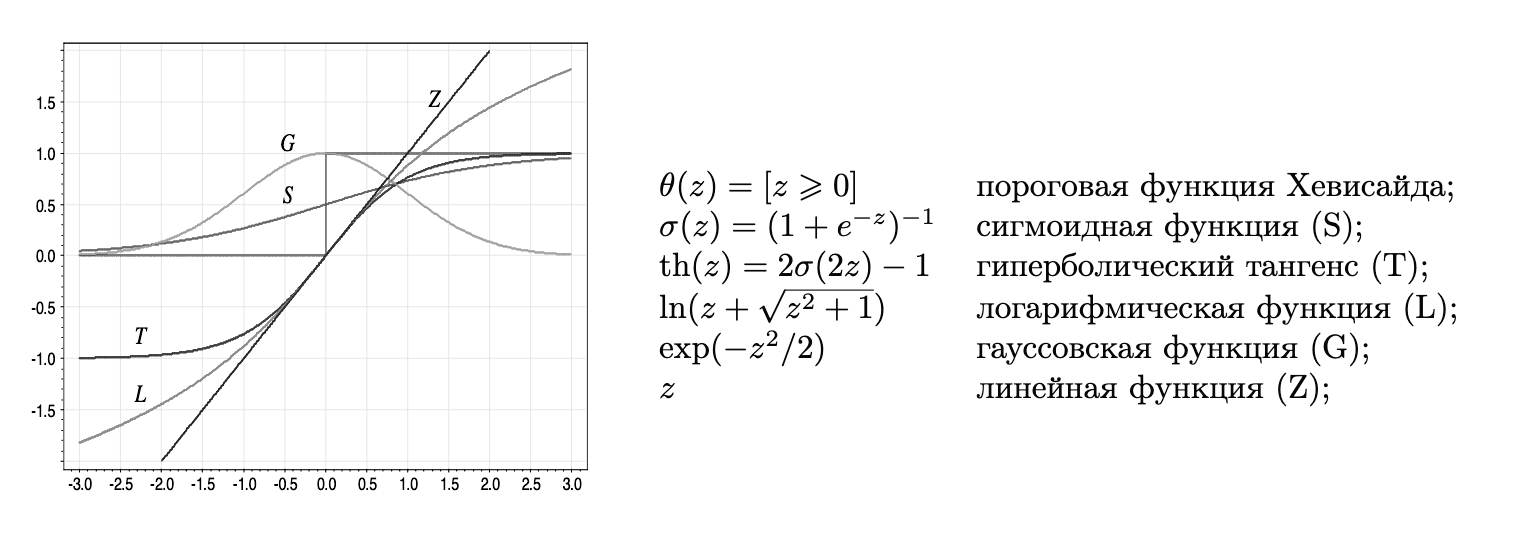
\includegraphics[scale=0.6]{pictures/activation.png}
                \caption{Активационные функции}
                \label{fig:my_label}
            \end{figure} 
        \par
        Если суммарный заряд превышает порог активации $w_0$, то нейрон возбуждается и выдает 1, иначе -1.\\ \\
        \newpage
        \paragraph
        {
        Autoencoder
        }
        \noindent\\
        
        Автоэнкодер -- нейронная сеть, обучающаяся не на отображение в пространство классов, а на самоотображение.\\
        
        \begin{figure}[h!]
                \centering
                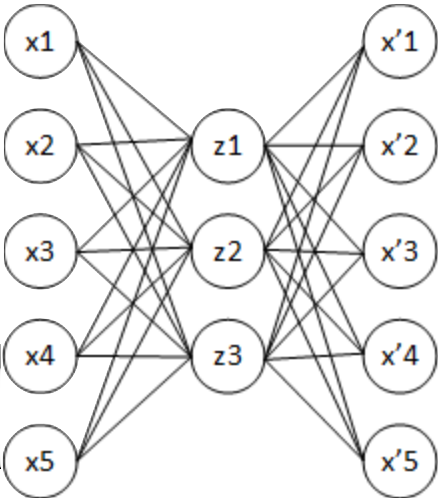
\includegraphics[scale=1]{pictures/autoencoder.png}
                \caption{Примитивный автоэнкодер}
                \label{fig:my_label}
            \end{figure} 
        \par\\
        
        Обучение автоэнкодера происходит путем минимизации ошибки между входным и выходным слоем. \\ \\
        Промежуточные слои автоэнкодера, в отличие от персептрона, должны иметь меньшую размерность, чем входной и выходной слои, для того, чтобы исключенить тривиальность решения.
    \newpage
    \section{Модель данных}
        Данные предоставлены в виде RAW сигналов преамбул с 5-ти различных устройств, расположенных в двух различных местах. \\
        Эти устройства:
        \begin{itemize}
            \item Lenovo
            \item Moto 8
            \item Pixel
            \item Tab 4
            \item Zen
        \end{itemize}\\
        
        Хранятся данные в формате .mat файлов, в структуре данных dict.\\ 
        Обращение к данным производится по полям "$X$" – для получения выборки, и "$y$" – для получения массива классов.
        
        \paragraph{Краткое описание датасета:}
        \begin{itemize}
            \item Приемник – ADALM PLUTO
            \item Передатчики – смартфоны
            \item 5 несбалансированных классов
            \item 2 различных канала
            \item 17281 преамбула
            \item 480 признаков
        \end{itemize}
        \begin{figure}[h!]
                \centering
                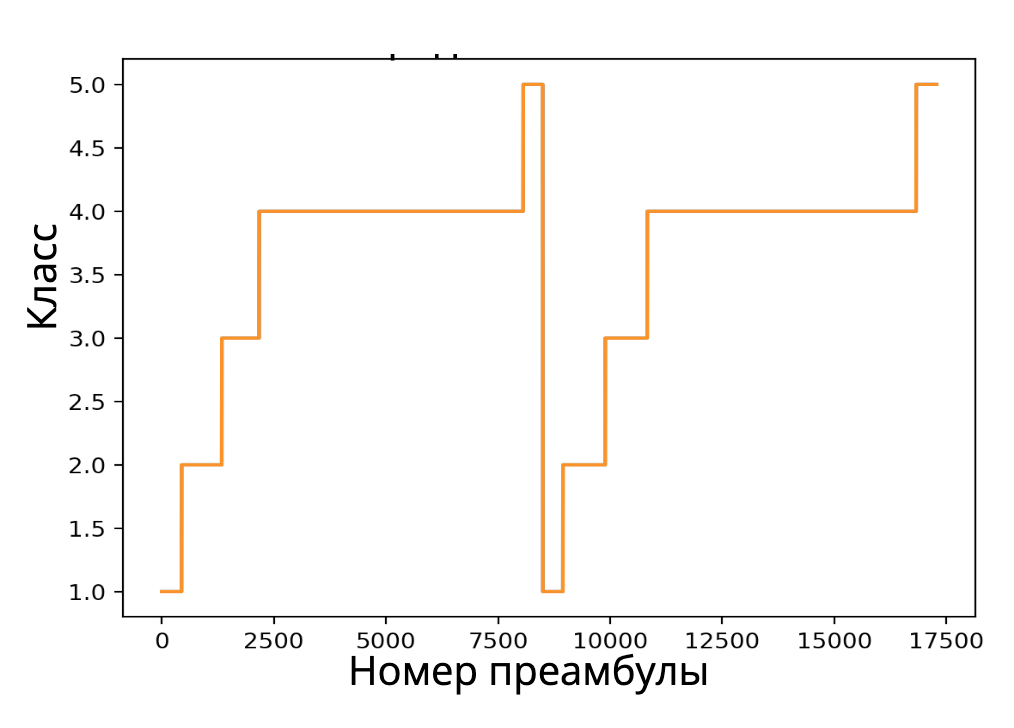
\includegraphics[scale=0.4]{pictures/target.png}
                \caption{График распределения классов}
                \label{fig:my_label}
            \end{figure} 
        \par

\chapter{Исследование решения}
\label{chap:research}

    \section{Описание эксперимента} \\ 
        \paragraph{Предобработка данных}
        \noindent 
        
        \noindent
        \begin{enumerate}
            \item Выделение преамбул из RAW сигналов
            \item Деление преамбул на поля
            \item Параллельная обработка полей преамбул:
            \begin{enumerate}
                \item FFT
                \item Модуль от преобразования Фурье
                \item Выделение значимых частей спектра
                \item Попарное вычитание частей спектра (последний элемент из первого и так далее)
            \end{enumerate}
            \item Конкатенация полученных разностей в один датасет
            \end{enumerate} 
            \begin{figure}[h!]
                \centering
                
\includegraphics[scale=0.5]{pictures/algh.png}
                \caption{Алгоритм предобработки данных}
                \label{fig:my_label}
            \end{figure} 
             \begin{figure}[h!]
            \centering
            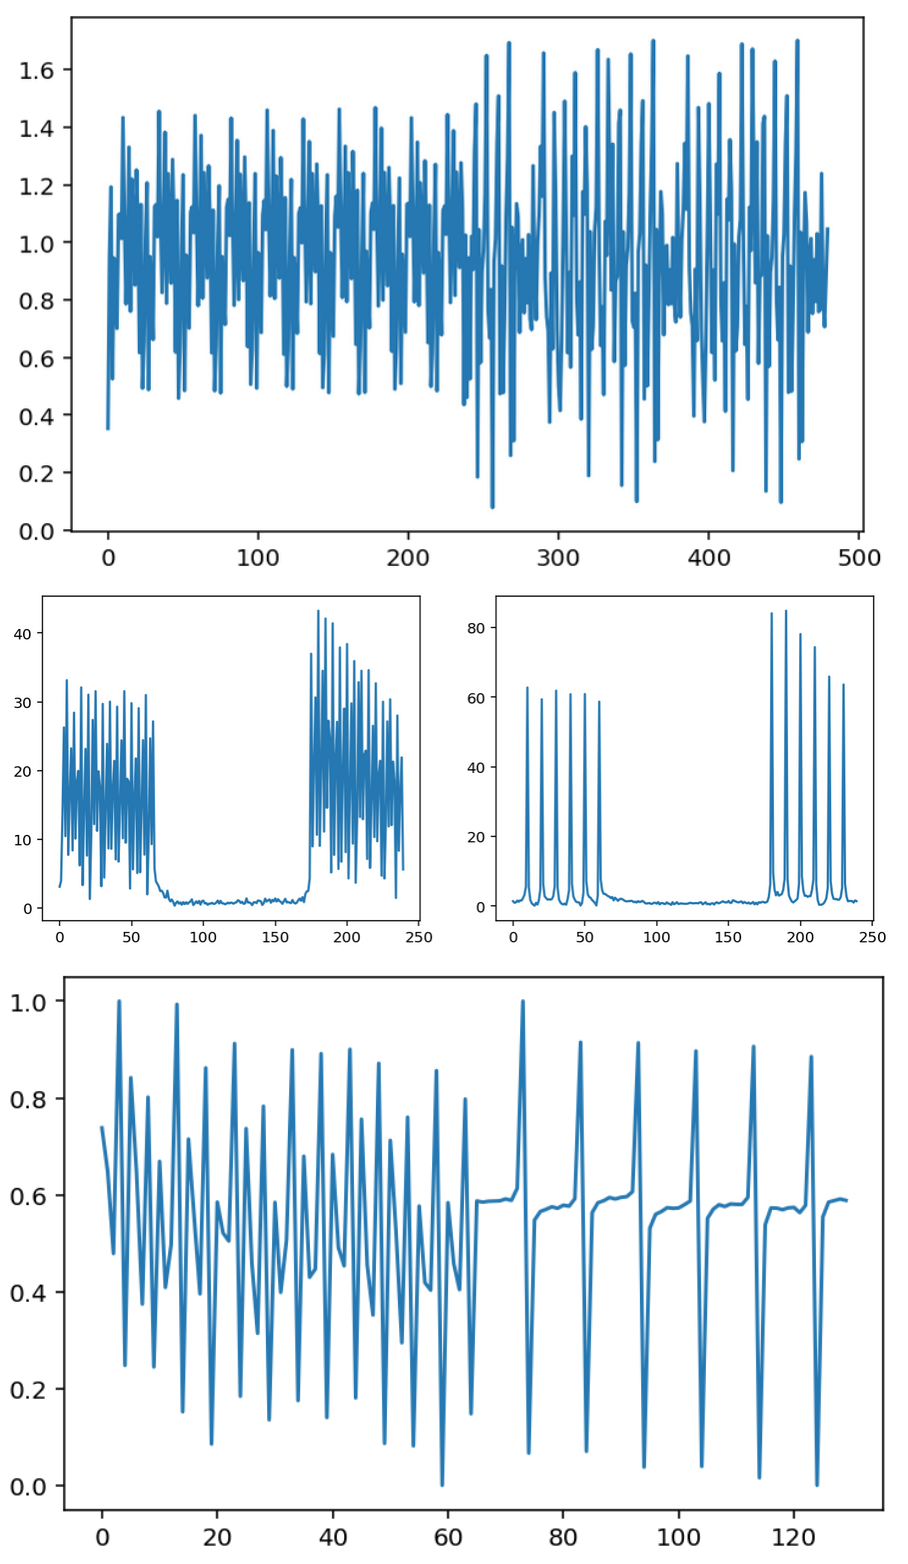
\includegraphics[scale=0.61]{pictures/preproc.png}
            \caption{Результаты обработки, соответствующие шагам 1, 2 и 4
            }
            \label{fig:my_label}
        \end{figure}
            \par
             
        \newpage
        \paragraph{Кодирование/отбор признаков}
        \noindent 
        
        \noindent
        \begin{enumerate}
            \item Отбор признаков с помощью Random Forest
            \begin{enumerate}
                \item Обучение Decision Tree, подбор гиперпараметров
                \item Построение Random Forest на основе обученного дерева решений
                \item Обучение Random Forest
                \item Вызов метода .feature\_importances\_
                \item Сортировка 
                \item Подбор оптимального количества признаков
                \item Оценка результата
            \end{enumerate}
            
            \item Уменьшение размерности признакового пространства с помощью встроенного в MATLAB автоэнкодера
            \item Построение автоэнкодера на основе библиотеки Keras
            \begin{enumerate}
                \item Выбор количества слоев и их размеров
                \item Выбор функций активации
                \item Подбор необходимой комбинации слоев и функций
                \item Оценка результата \\
            \end{enumerate}
            \item TSNE –– проекция выборки на двухмерное пространство для визуализации, а также получения новой информации о данных
            \begin{figure}[h!]
                \centering
                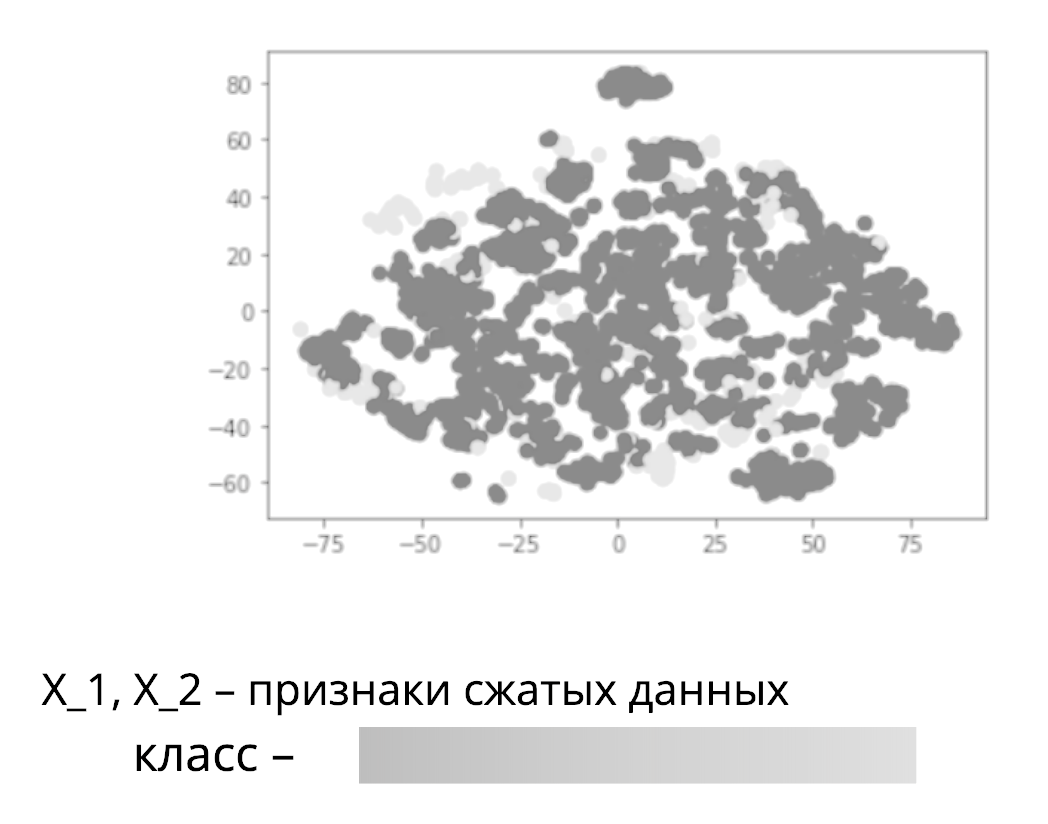
\includegraphics[scale=0.5]{pictures/tsne.png}
                \caption{TSNE
                }
                \label{fig:my_label}
            \end{figure} 
        \end{enumerate} 
        \newpage
        \paragraph{Классификация}
        %сценарий: данные, величины, последовательность действий, гипотезы
        \noindent 
        
        \noindent
        \begin{enumerate}
            \item Decision Tree
            \begin{enumerate}
                \item Кросс-валидация
                \item Обучение
                \item Оценка результатов
            \end{enumerate}
            \item Random Forest
            \begin{enumerate}
                \item Кросс-валидация
                \item Обучение
                \item Оценка результатов
            \end{enumerate}
            \item Multilayer Perceptron
            \begin{enumerate}
                \item Кросс-валидация
                \item Обучение
                \item Оценка результатов
            \end{enumerate}
            \item CatBoostClassifier
            \begin{enumerate}
                \item Кросс-валидация
                \item Обучение
                \item Оценка результатов
            \end{enumerate}
        \end{enumerate}
        
        \paragraph{Адаптация алгоритма}
            \begin{enumerate}
                \item Алгоритм для адаптации – Multilayer Perceptron, как максимально подходящий требованиям к решению
                \item Данные берутся по 300 отсчетов --  batch
                \item Обучение происходит постепенно -- N epochs
                \item После достижения локального взвешенного максимума подается только тестовая выборка
            \end{enumerate}
        
        \newpage
        \paragraph{Технические характеристики} 
\\
         \begin{itemize}
             \item MacBook Pro 13 2015
             \item Процессор 2.7 GHz 2-ядерный Intel Core i5
             \item Память 8 ГБ 1867 MHz DDR3 \\
         \end{itemize}
        %методика измерения: хар-ки пк, инструменты измерения
        \paragraph{Программные средства}
        \begin{itemize}
             \item Язык программирования Python 3.10
             \item Jupyter notebook
             \item Jupyter lab
             \item Atom + Terminal
             \item Graphix
             \item MATLAB 
             \item Библиотеки:
             \begin{itemize}
                 \item Scikit-learn
                 \item Numpy
                 \item Pandas
                 \item MatPlotLib
                 \item SciPy
                 \item TensorFlow
                 \item Keras
                 \item PyTorch
                 \item Seaborn
                 \item CatBoost
                 \item CatBoostClassifier \\
             \end{itemize}
         \end{itemize}
        %используемые программные средства
        
    \newpage
    \section{Результаты}
        \paragraph{Выбор признакового описания}
        \noindent 
        
        
        \begin{table}[h!]
        \centering
        \resizebox{550}{!}{
        \begin{tabular}{l|ccccl|cccl|cccl|lll}
        \cline{2-14}
                   & \multicolumn{5}{c|}{Preambule}                                                                                               & \multicolumn{4}{c|}{L-STF}                                                                      & \multicolumn{4}{c|}{L-LTF}                                                                      &  &  &  \\ \cline{2-14}
                   & \multicolumn{1}{l|}{real}  & \multicolumn{1}{l|}{imag}  & \multicolumn{1}{l|}{abs}   & \multicolumn{1}{l|}{angle} & abs(fft) & \multicolumn{1}{l|}{real}  & \multicolumn{1}{l|}{imag}  & \multicolumn{1}{l|}{abs}   & abs(fft) & \multicolumn{1}{l|}{real}  & \multicolumn{1}{l|}{imag}  & \multicolumn{1}{l|}{abs}   & abs(fft) &  &  &  \\ \cline{1-14}
                    \multicolumn{1}{|l|}{Accuracy} & \multicolumn{1}{c|}{0.732} & \multicolumn{1}{c|}{0.733} & \multicolumn{1}{c|}{0.842} & \multicolumn{1}{c|}{0.702} & 0.828    & \multicolumn{1}{c|}{0.734} & \multicolumn{1}{c|}{0.731} & \multicolumn{1}{c|}{0.838} & 0.785    & \multicolumn{1}{c|}{0.725} & \multicolumn{1}{c|}{0.728} & \multicolumn{1}{c|}{0.836} & 0.822    &  &  &  \\ \cline{1-14}
                    \multicolumn{1}{|l|}{F1-score} & \multicolumn{1}{c|}{0.667} & \multicolumn{1}{c|}{0.663} & \multicolumn{1}{c|}{0.823} & \multicolumn{1}{c|}{0.597} & 0.803    & \multicolumn{1}{c|}{0.668} & \multicolumn{1}{c|}{0.664} & \multicolumn{1}{c|}{0.819} & 0.744    & \multicolumn{1}{c|}{0.646} & \multicolumn{1}{c|}{0.653} & \multicolumn{1}{c|}{0.812} & 0.796    &  &  &  \\ \cline{1-14}
        \end{tabular}}
        \caption{}
        \label{tab:my-table}
        \end{table}
        В Таблице 1 находятся результаты оценки Random Forest различных преобразований данных.
        \begin{table}[h!]
            \begin{tabular}{l|c|c|c|l}
                \cline{2-4}
                                               & L-STF + L-LTF & L-STF & L-LTF &  \\
                                               \cline{1-4}
                \multicolumn{1}{|l|}{Accuracy} & 0.85          & 0.83  & 0.84  &  \\ \cline{1-4}
                \multicolumn{1}{|l|}{F1-score} & 0.83          & 0.81  & 0.83  &  \\ \cline{1-4}
            \end{tabular}
            \caption{Оценка для L-STF, L-LTF и их суммы}
            \label{tab:my-table}
        \end{table}
        
        Таблица 2 – сравнительная таблица F1-score и Accuracy на классификаторе Random Forest для полей L-STF, L-LTF и их суммы, прошедших выбранную схему преобразования.\\ Очевидно, что L-LTF вносит больший вклад в решение задачи классификации, чем L-STF, но их сумма показывает большую точность.
        
        \begin{figure}[h!]
            \centering
            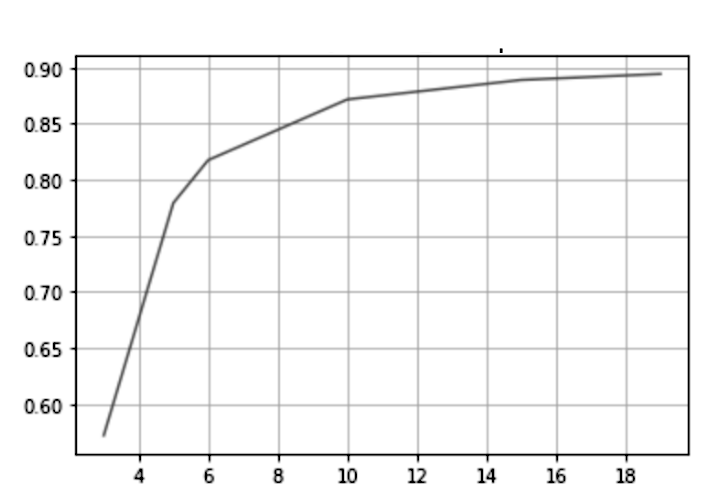
\includegraphics[scale=1]{pictures/acc_nf.png}
            \caption{Точность от количества признаков
            }
            \label{fig:my_label}
        \end{figure} 
        
        На рис. 15 изображена зависимость Accuracy от количества признаков в выборке. Эти признаки отобраны по значимости, рассчитанной Random Forest. \\Можно заметить, что начиная с 10 признаков Accuracy меняется незначительно, то есть это значение оптимально.
        
        \newpage
        \begin{figure}[h!]
            \centering
            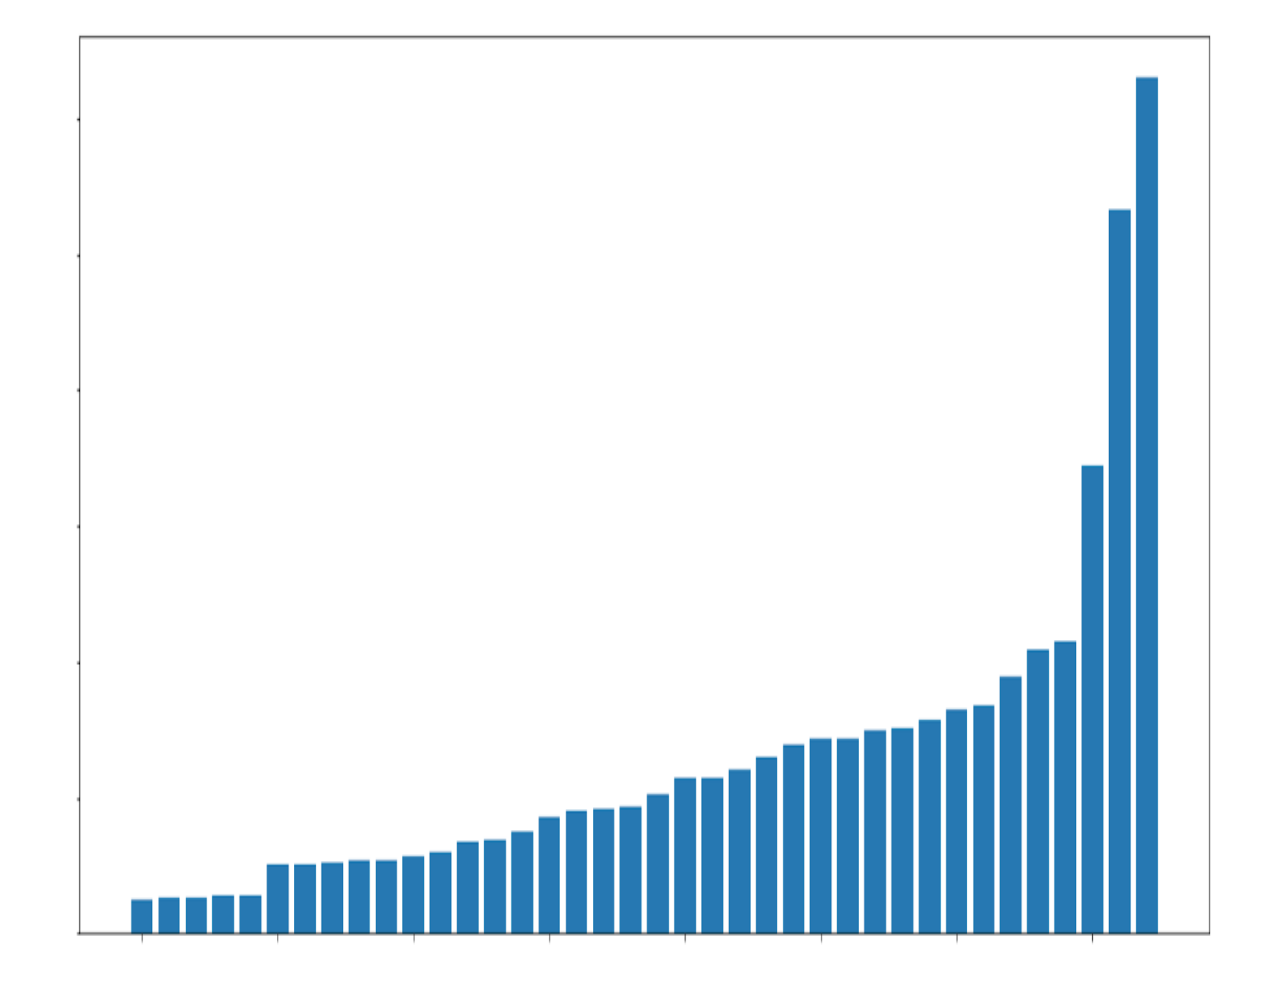
\includegraphics[scale=0.5]{pictures/RF-ff.png}
            \caption{Средний вклад в изменение энтропии от признака
            }
            \label{fig:my_label}
        \end{figure} 
        
        На рис. 16 изображено распределение признаков выборки по их значимости, рассчитанной Random Forest.\\ Признаки расположены в порядке возрастания значимости -- среднего вклада в изменение энтропии при построении дерева.\\
        
        \paragraph{Точность классификации \\} \\
        \noindent
        \begin{table}[h!]
        \begin{tabular}{l|l|l|l}
        \cline{2-3}
                                                          & Accuracy & F1-score &  \\ \cline{1-3}
        \multicolumn{1}{|l|}{Decision tree}               & 0.81     & 0.73     &  \\ \cline{1-3}
        \multicolumn{1}{|l|}{Random forest}               & 0.86     & 0.78     &  \\ \cline{1-3}
        \multicolumn{1}{|l|}{CatBoost Classifier}         & 0.95     & 0.88     &  \\ \cline{1-3}
        \multicolumn{1}{|l|}{Autoencoder + Random forest} & 0.85     & 0.83     &  \\ \cline{1-3}
        \multicolumn{1}{|l|}{Autoencoder + MLP}           & 0.92     & 0.91     &  \\ \cline{1-3}
        \multicolumn{1}{|l|}{Autoencoder + CatBoost}      & 0.91     & 0.90     &  \\ \cline{1-3}
        \end{tabular}
        \caption{Таблица классификаторов}
        \label{tab:my-table}
        \end{table}
        В таблице 3 указаны оценки классификаторов в различных конфигурациях. \\Можно заметить, что самые примитивные классификаторы – DT и RF дают неплохой результат, но не полностью отвечают сформулированным требованиям. Лучшими комбинациями являются Autoencoder+MLP и Autoencoder+CatBoost.
        \newpage
        \paragraph{Сравнительный анализ}
        \noindent\\
        Рассмотрим подробнее классификаторы CatBoostClassifier и MLPClassifier.
        
        \begin{figure}[h!]
                \centering
                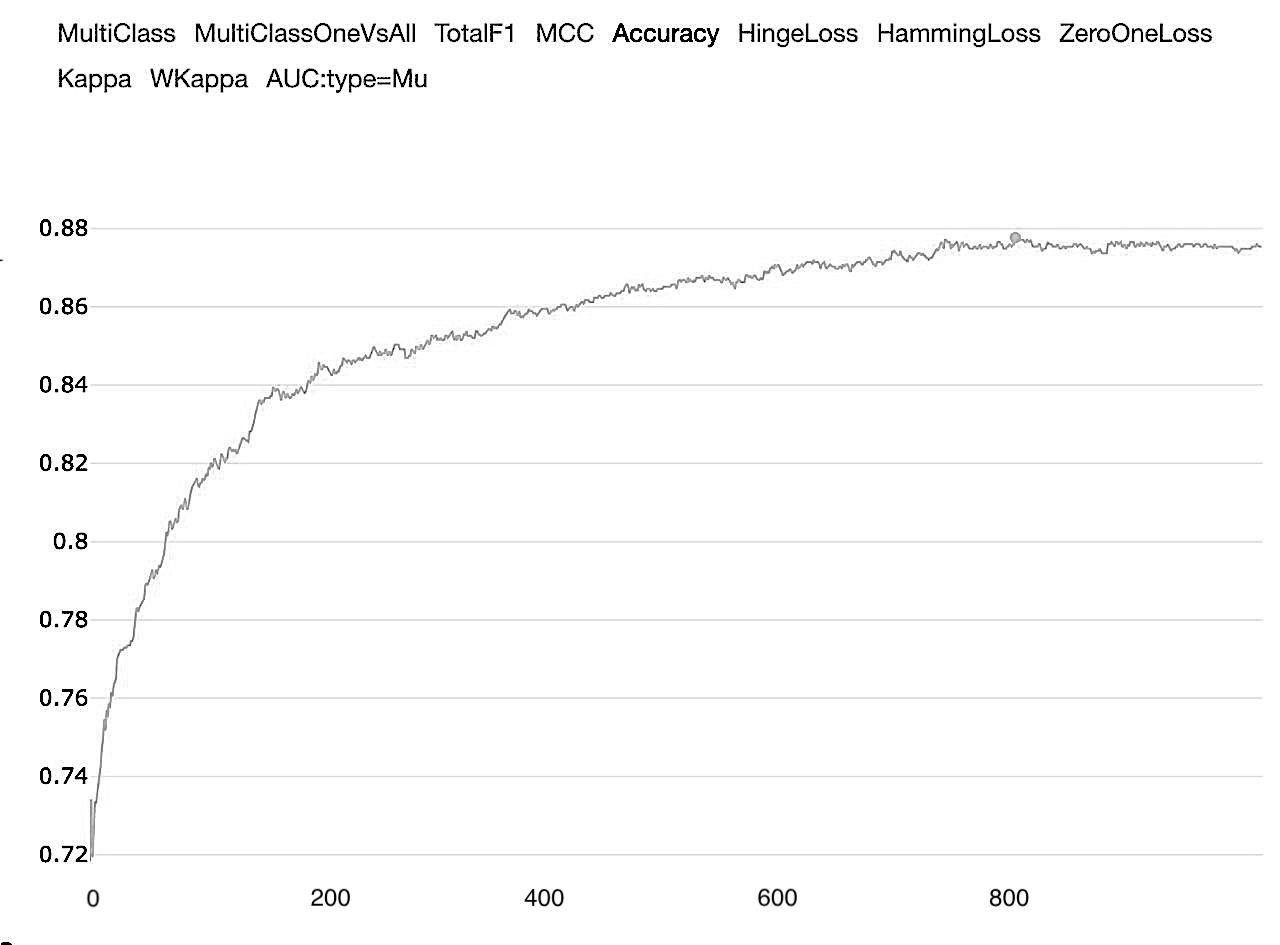
\includegraphics[scale=0.2]{pictures/2022-06-21 02.22.10.jpg}
                \caption{CatBoostClassifier
                }
                \label{fig:my_label}
            \end{figure} 
        \begin{figure}[h!]
                \centering
                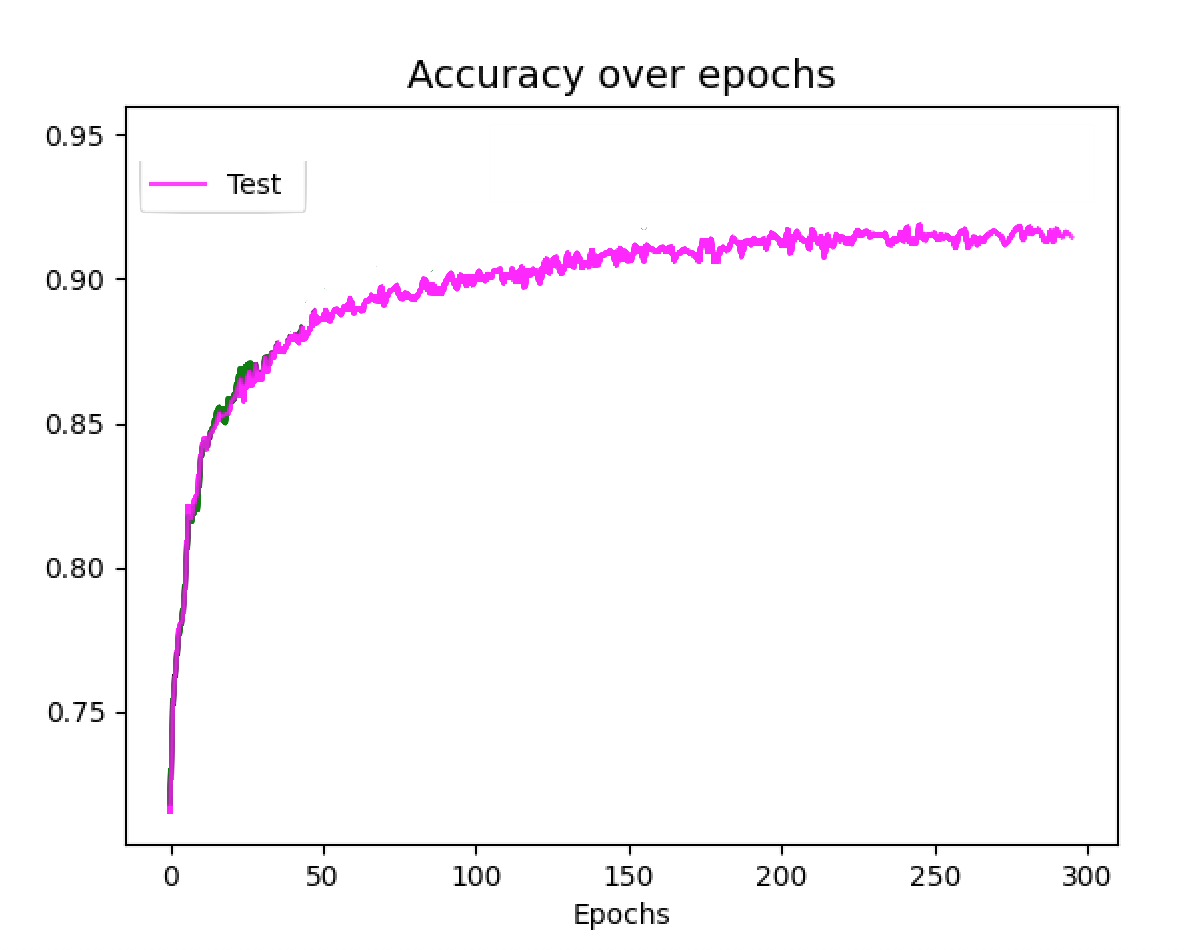
\includegraphics[scale=0.5]{pictures/realtime.png}
                \caption{Multylayer Perceptrone
                }
                \label{fig:my_label}
            \end{figure} 
            Оба алгоритма сходятся, CatBoost – к 0.88, а MLP – к 0.91, при этом оба работают в режиме реального времени.
        \noindent
        \paragraph{Выводы}
        
        \begin{itemize}
            \item Лучшее признаковое пространство получено преобразованиями+автоэнкодером
            \item Самую высокую точность показал многослойный персептрон
            \item Задача классификации решается композицией вышеназванных алгоритмов в онлайн-режиме со стабильной точностью
        \end{itemize}
        \noindent
        
\chapter{Заключение\\}
\label{chap:summary}
    \paragraph{Цель}
    \noindent\\
    В ходе данной работы была достигнута поставленная цель -- разработан алгоритм, позволяющий в реальном времени идентифицировать устройства с точностью >90\%.
    \paragraph{Задачи}
    \noindent
    
    \noindent
    Был произведен анализ предметной области, исследованы алгоритмы понижения размерности и классификации, а также различные способы адаптации решения к работе в реальном времени.
    
    \begin{itemize}
	    \item Подобрано эффективное признаковое описание:
	    \begin{itemize}
	        \item С помощью преобразований сигнала -- последовательного вычитания друг из друга симметричных частей спектра, полученного после взятия модуля от быстрого преобразования Фурье от частей преамбулы и дальнейшего их объединения, -- была уменьшена размерность с 480 признаков до 130 с потерей точности менее, чем 0.5\%.
	        \item Смоделирован с помощью библиотеки Keras и обучен автоэнкодер, уменьшающий размерность с 130 признаков до 20 с потерей точности менее, чем 1.5\%.
	    \end{itemize}
	    \item Произведено сравнение и подбор классификаторов:
	    \begin{itemize}
	        \item Модели, основанные на решающих деревьях дали точность 0.8-0.9, но показали себя немасштабируемыми: для того, чтобы давать хороший результат, им необходимо обучиться на большом объеме данных.
	        \item CatBoost от Yandex хорошо показала себя как модель, имеющая хорошую вариативность гиперпараметров и метрик, а также, даже без оптимизации параметров, CatBoost дает точность >0.85.
	        \item Модель MLP, схожая по устройству с автоэнкодером, показала лучший результат – Accuracy = 0.92.\\
	    \end{itemize}
	    \item Разработан и реализован алгоритм онлайн-классификации:
	    \begin{itemize}
	        \item В основу алгоритма легли Autoencoder и Multilayer Perceptrone
	        \item Обучение алгоритма происходит последовательно по эпохам на рандомизированных данных
	        \item Алгоритм имеет возможность сохранения модели для дальнейшего использования
	        \item Модель не требует большого количества памяти для сохранения
	    \end{itemize}
	\end{itemize}\\ 
    

\backmatter
\begin{thebibliography}{99}
    
    \bibitem{0}
        Merchant, K., Revay, S., Stantchev, G., et al.: \\Deep learning for RF device fingerprinting in cognitive communication networks. \\\emph{IEEE J. Sel. Top. Signal Process.}, 12(1), 160–167 (2018)
    \bibitem{2}   
        Danev, B., Capkun, S.: \\Transient-based identification of wireless sensor nodes. \\\emph{ International Conference on Information Processing in Sensor Networks IEEE 2009}, pp. 25–36. IEEE (2009)
    \bibitem{5}   
        Toonstra, J., Kinsner, W.: \\Transient analysis and genetic algorithms for classification. \\\emph{ Conference Proceedings of the IEEE Communications, Power, and Computing IEEE 1995}, WESCANEX 95, vol. 2, pp. 432–437. IEEE (1995)
    \bibitem{7}    
        Polak, A.C., Dolatshahi, S., Goeckel, D.L.: \\Identifying wireless users via transmitter imperfections. \\\emph{IEEE J. Sel. Areas Commun.} 29(7), 1469–1479 (2011)
    \bibitem{16}
        Novikoff A. B. J. :\\
        On convergence proofs on perceptrons \\
        \emph{Proceedings of the Symposium on the Mathematical Theory of Automata.} \\
         Vol. 12.  Polytechnic Institute of Brooklyn, 1962.  Pp. 615–622
    \bibitem{13}
        Nigmatullin R.R., Vorobev A.S.: \\The “Universal” Set of Quantitative Parameters for Reading of the Trendless Sequences\\  \emph{ Fluctuation and Noise Letters}, 18(04), 2019
    \bibitem{3}   
        Li, Z., Xu, W., Miller, R., et al.: \\Securing wireless systems via lower layer enforcements. \\\emph{ ACM Workshop on Wireless Security ACM}, pp. 33–42. ACM (2006)
    \bibitem{8}    
        К. В. Воронцов \\Математические методы обучения по прецедентам
(теория обучения машин), \\\emph{В рамках курса лекций по машинному обучению,} 2013
    \bibitem{9}    
        Nguyen, N.T., Zheng, G., Han, Z., et al.: \\Device fingerprinting to enhance wireless security using nonparametric Bayesian method. \\\emph{ Proceedings IEEE, INFOCOM 2011, IEEE 2011}, vol. 34, pp. 1404–1412. IEEE (2011)
     \bibitem{11}
        A. Selcuk Uluagac, Sakthi V. Radhakrishnan, Cherita Corbett, Antony Baca, Raheem Beyah:\\ A passive technique for fingerprinting wireless devices with Wired-side Observations.\\ \emph{Conference on Communications and Network Security (CNS)} 2013 IEEE
    \bibitem{6}    
        Gao, K., Corbett, C., Beyah, R.: \\A passive approach to wireless device fingerprinting. \\\emph{ IEEE/IFIP International Conference on Dependable Systems and Networks}, IEEE 2010, pp. 383–392. IEEE (2010)
    \bibitem{12}
        Marco Tulio Ribeiro, Sameer Singh, and Carlos Guestrin:  \\"Why Should I Trust You?": Explaining the Predictions of Any Classifier. \\ \emph{ In Proceedings of the 22nd ACM SIGKDD International Conference on Knowledge Discovery and Data Mining (KDD '16). Association for Computing Machinery}, New York, NY, USA, 1135–1144. 2016.
    \bibitem{4}   
        Liang, X., Greenstein, L., Mandayam, N., et al.: \\Fingerprints in the ether: using the physical layer for wireless authentication. \\\emph{ IEEE International Conference on Communications IEEE}, pp. 4646–4651. IEEE (2009)
    \bibitem{14}
        Minsky M., Papert S.:\\
        Perceptrons: an Introduction to Computational Geometry. \\
        \emph{MIT Press}, 1968.
    \bibitem{15}
        LeCun Y., Denker J., Solla S., Howard R. E., Jackel L. D.:\\
        Optimal brain damage \\
        \emph{Advances in Neural Information Processing Systems II} \\
        Ed. by D. S. Touretzky. \\
        San Mateo, CA: Morgan Kauffman, 1990.
    \bibitem{1}
        Polak, A.C., Goeckel, D.L.: \\Wireless device identification based on RF oscillator imperfections. \\\emph{ IEEE International Conference on Acoustics, Speech and Signal Processing IEEE}, vol. 10, pp. 2492–2501. IEEE (2014)
    \end{thebibliography}
\end{document}